\documentclass[12pt, twoside]{article}
\usepackage[francais]{babel}
\usepackage[T1]{fontenc}
\usepackage[latin1]{inputenc}
\usepackage[left=7mm, right=7mm, top=7mm, bottom=7mm]{geometry}
\usepackage{float}
\usepackage{graphicx}
\usepackage{array}
\usepackage{multirow}
\usepackage{amsmath,amssymb,mathrsfs} 
\usepackage{soul}
\usepackage{textcomp}
\usepackage{eurosym}
 \usepackage{variations}
\usepackage{tabvar} 

\begin{document}

\begin{center}
\textbf{Exercices sur les nombres relatifs}
\end{center}


\begin{tabular}{cc}
\begin{minipage}{9cm}

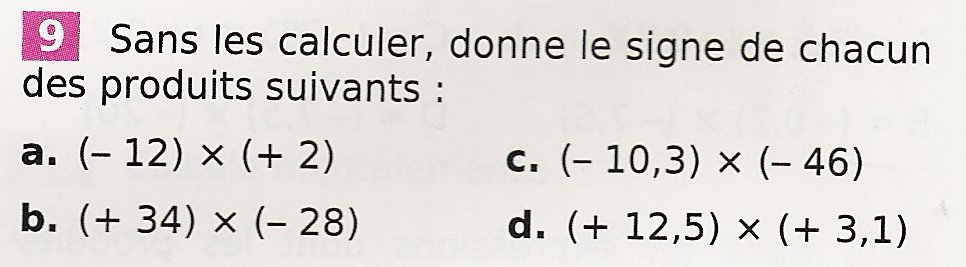
\includegraphics[width=7cm]{images/ex9p15.jpg}

\enskip

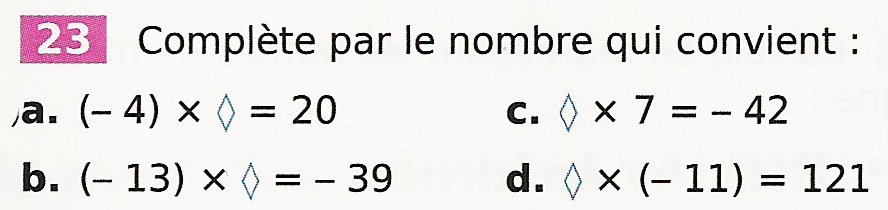
\includegraphics[width=7cm]{images/ex23p16.jpg}

\enskip

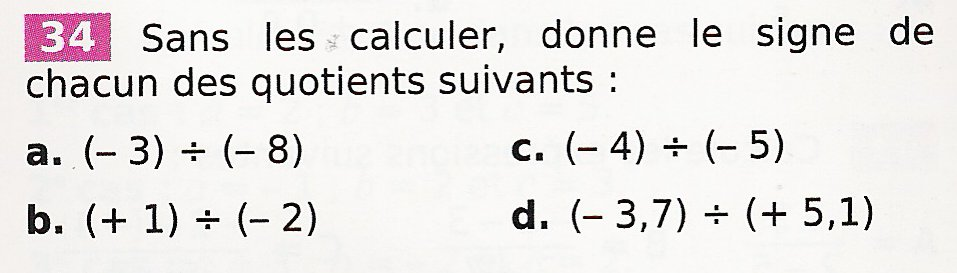
\includegraphics[width=7cm]{images/ex34p17.jpg}

\enskip

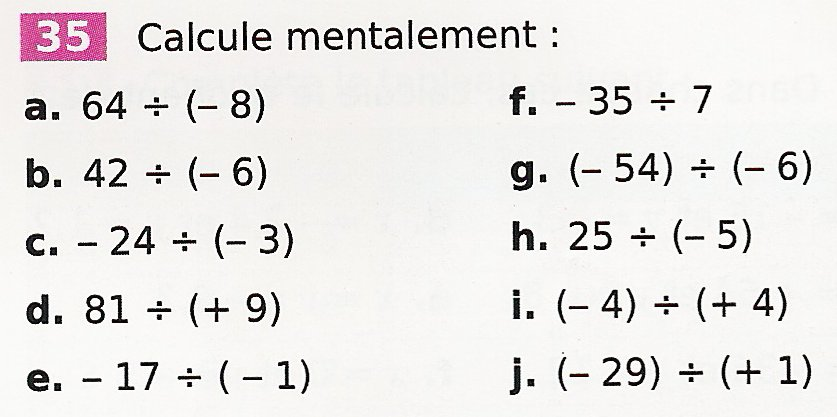
\includegraphics[width=6cm]{images/ex35p17.jpg}


\enskip

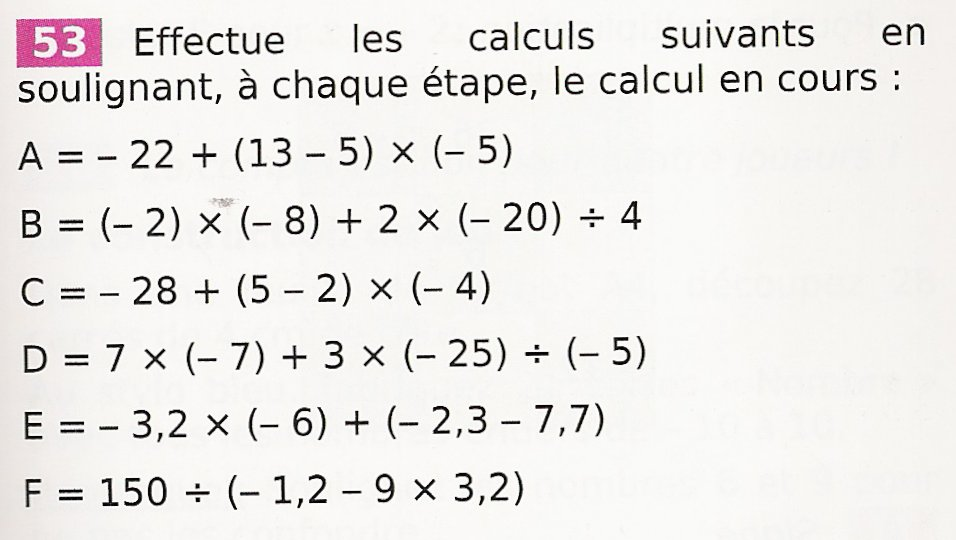
\includegraphics[width=7cm]{images/ex53p19.jpg}

\enskip

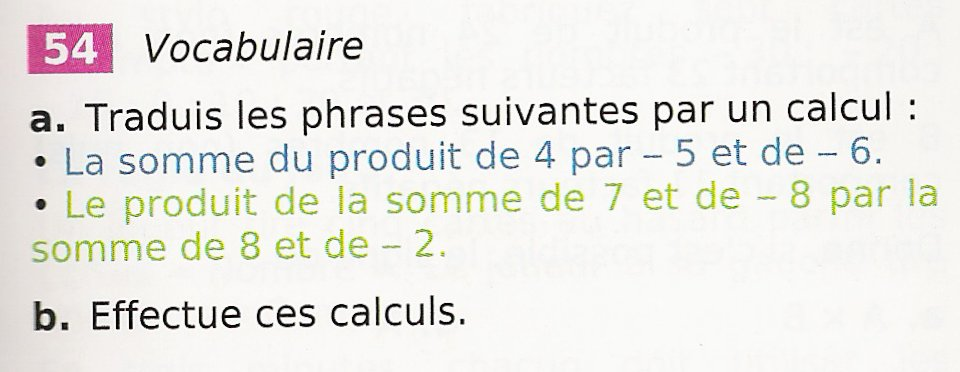
\includegraphics[width=7cm]{images/ex54p19.jpg}

\enskip

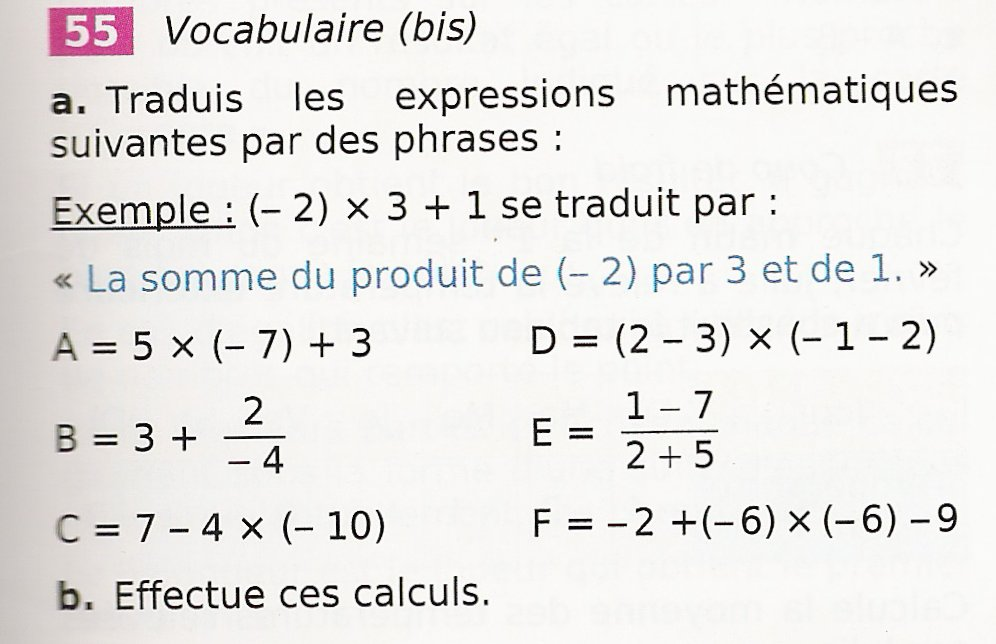
\includegraphics[width=7cm]{images/ex55p19.jpg}

\end{minipage}
&
\begin{minipage}{9cm}

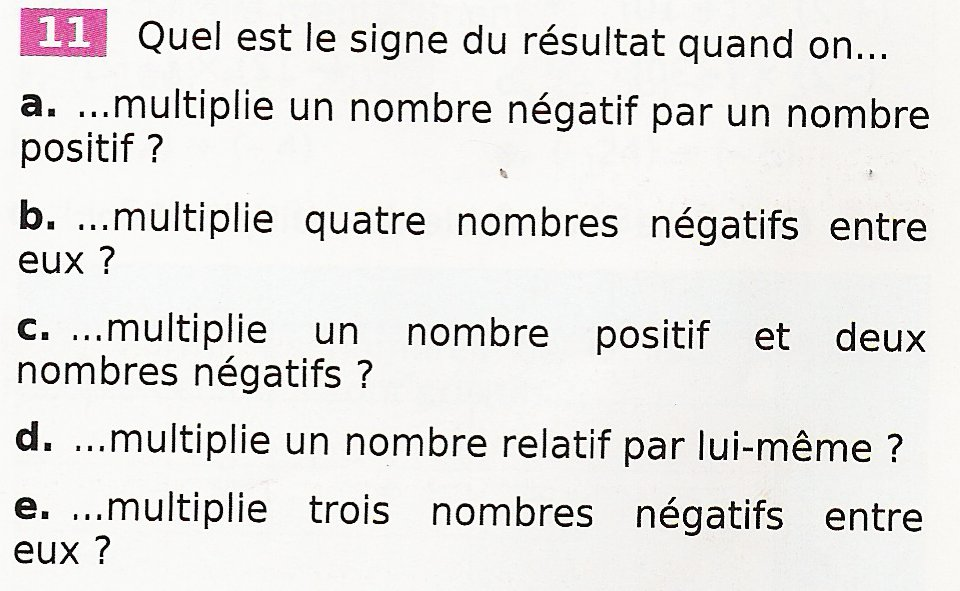
\includegraphics[width=7cm]{images/ex11p15.jpg}

\enskip

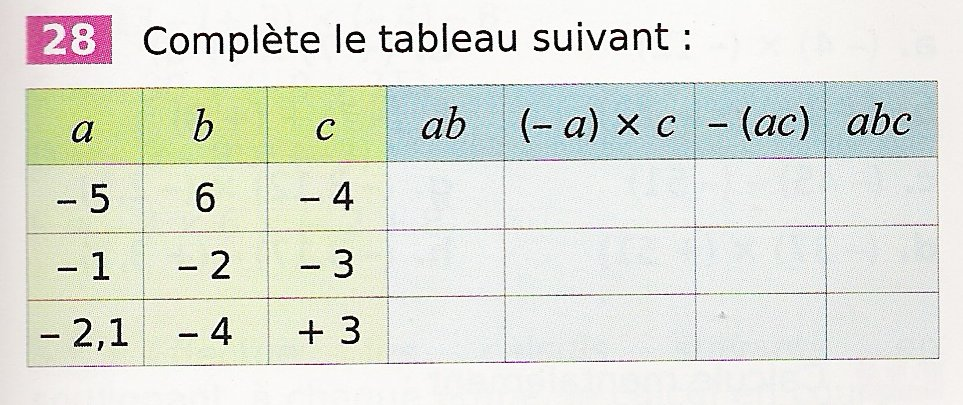
\includegraphics[width=7cm]{images/ex28p17.jpg}

\enskip

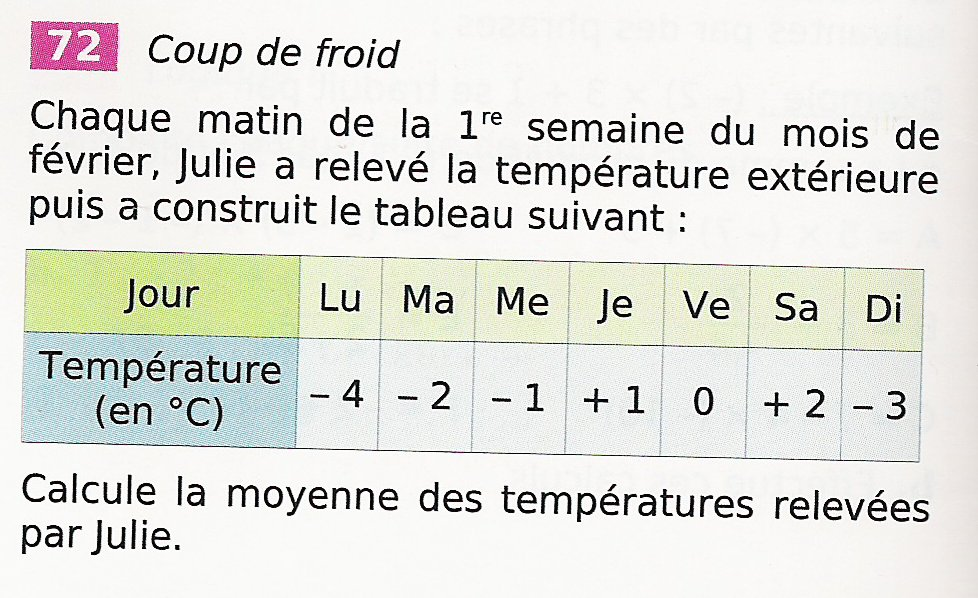
\includegraphics[width=7cm]{images/ex72p20.jpg}

\enskip

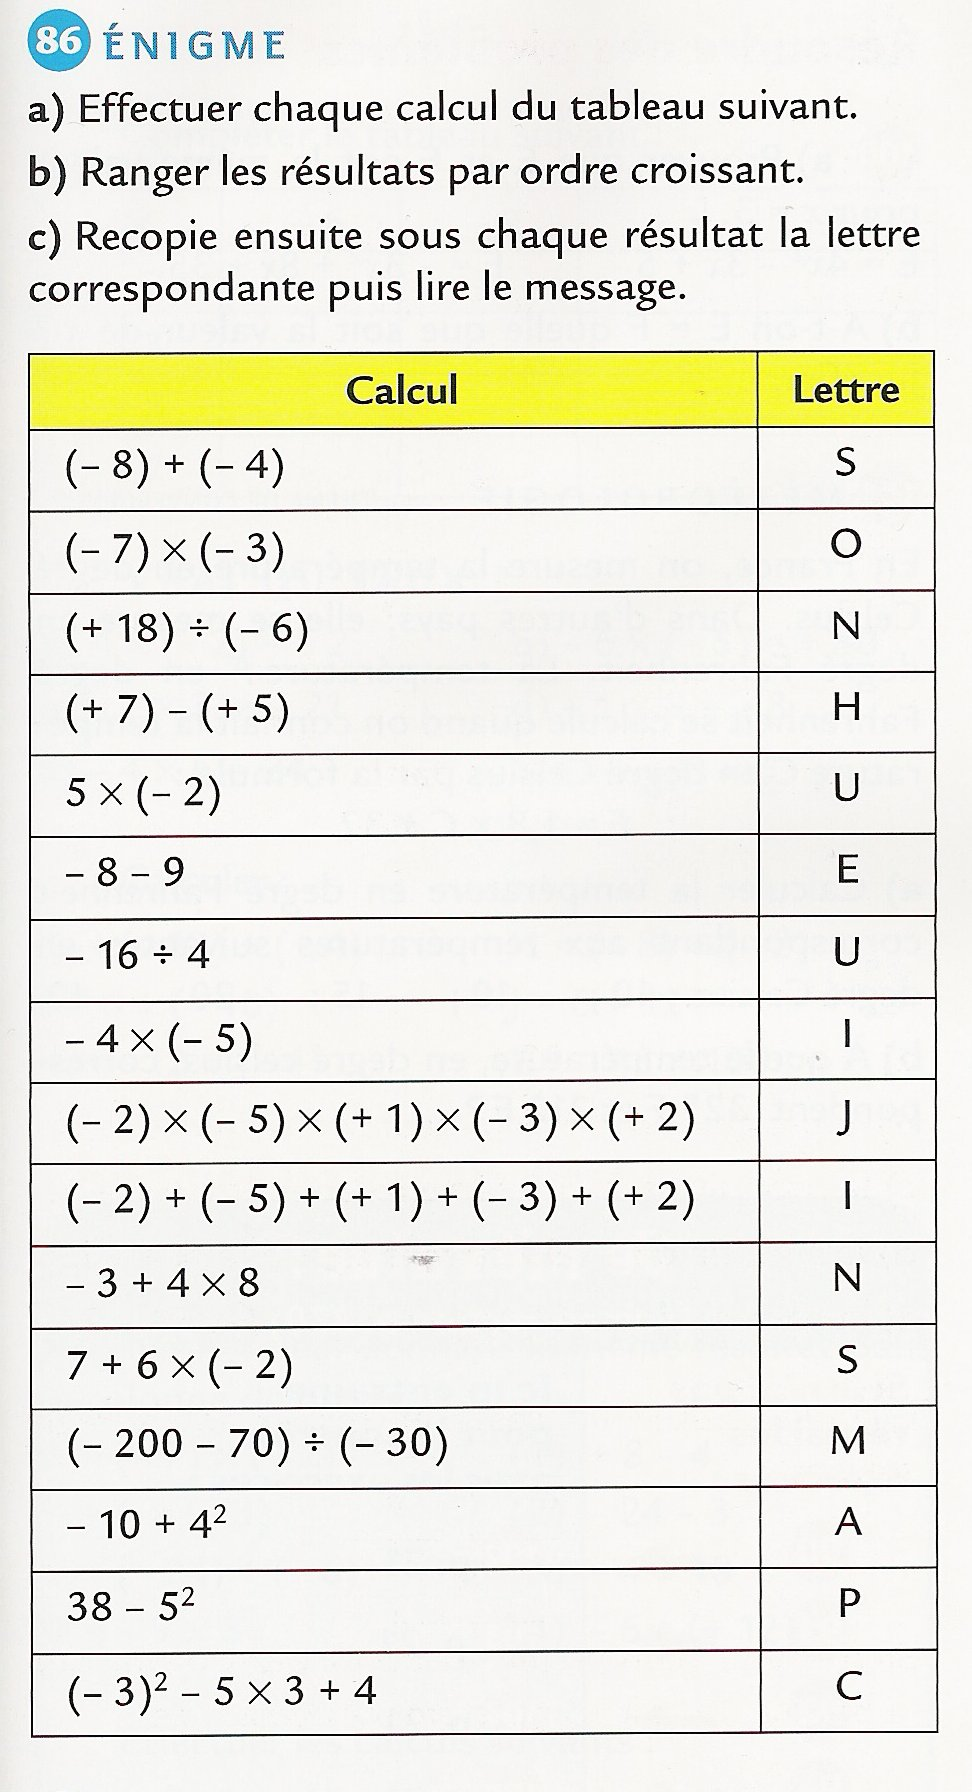
\includegraphics[width=7cm]{images/pb.jpg}
\end{minipage}
\end{tabular}



















 




\end{document}
